\documentclass[xcolor=dvipsnames]{beamer}
\usepackage[T1]{fontenc}
\usepackage[utf8]{inputenc}
\usepackage[english,slovak]{babel}

\usepackage{amsmath}
\usepackage{amsthm}
\usetheme{Pittsburgh}
\useoutertheme{shadow}

\usepackage{graphicx}
\usepackage{caption}
\usepackage{subcaption}

\usepackage[]{algorithm2e}
\usepackage{listings}
 \setbeamercovered{transparent}
 \usepackage{cuted}
\usepackage[export]{adjustbox}



\usepackage{lipsum}

\newcommand\Wider[2][3em]{%
\makebox[\linewidth][c]{%
  \begin{minipage}{\dimexpr\textwidth+#1\relax}
  \raggedright#2
  \end{minipage}%
  }%
}

%-------------------------------------------------------------------------------------
\title{\bf Monte Carlo localisation \\ using particle filter}
\author{Michal CHOVANEC}


%\setbeamertemplate{footline}[frame number]{}
\setbeamertemplate{navigation symbols}{}



\date[EURP]{\it Januray 2018}
\begin{document}

\begin{frame}
\titlepage
\end{frame}



\begin{frame}{\bf Problem formulation}

Robot localisation on known map

\begin{itemize}
  \item map, $\hat{o} = m(\hat{x}, \hat{y}) = m(\hat{r})$
  \item position change, $dr = (dx, dy) + noise$
  \item observation, $o(x, y) = o(r)$
\end{itemize}



\begin{figure}
\centering
\begin{minipage}{.5\textwidth}
  \centering
  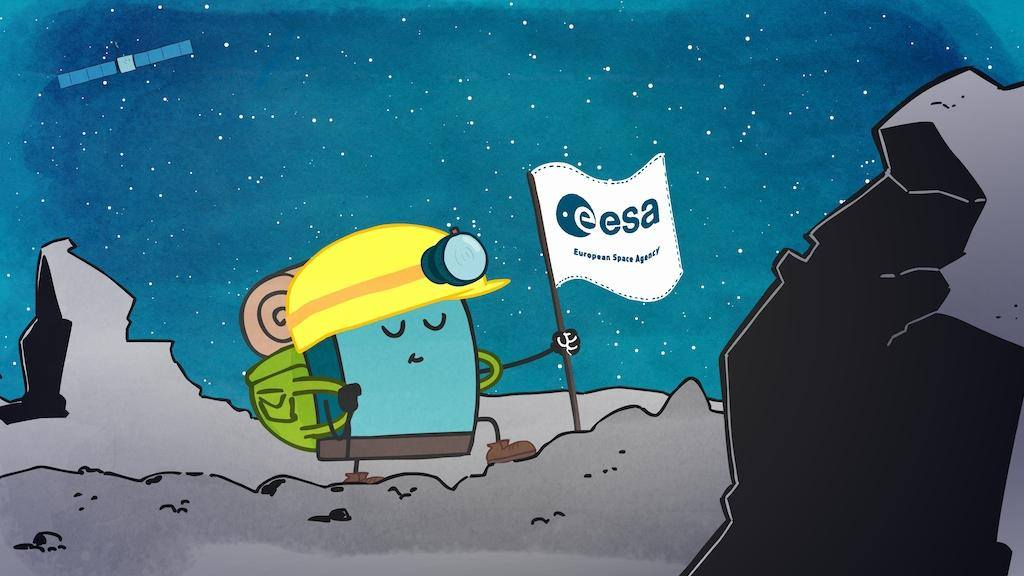
\includegraphics[scale=0.15]{../pictures/philae_esa.jpg}
\end{minipage}%
\begin{minipage}{.5\textwidth}
  \centering
  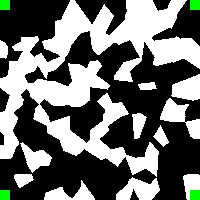
\includegraphics[scale=0.5]{../pictures/my_map.png}
\end{minipage}
\end{figure}


\end{frame}




\begin{frame}{\bf Particle filter - initialization}

Generate tons of random hypothesis -> particles \\
Particle : {\bf position} + {\bf weight} \\

\begin{figure}[htbp]
  \centering
   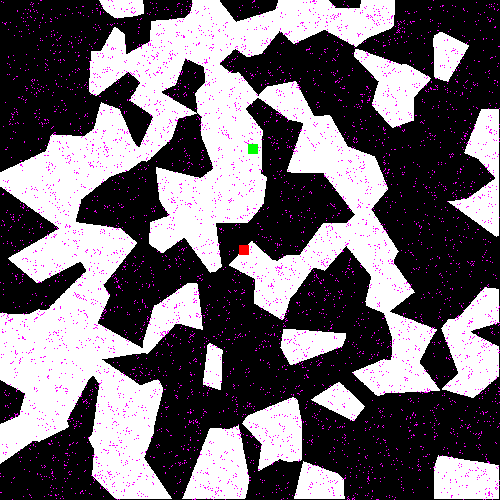
\includegraphics[scale=0.27]{../pictures/particles.png}
\end{figure}


\end{frame}



\begin{frame}{\bf Particle filter - algorithm}


\begin{algorithm}[H]
 \KwData{{\color{purple} map}, {\color{red}dr}, {\color{green} observation}}
 \KwResult{position R}
 initialization  \\
                 {\color{red}$P_r$} = random particles positions \\
                 {\color{blue}$P_w$} = only fist time init particles weights to zero \\
                  R = 0 \\
 MoveParticles({\color{red}$P_r$}, {\color{red}dr}) \\
 {\color{blue}$P_w$} = ComputeWeights({\color{green} observation}, ${\color{purple}map}({\color{red}P_r})$,  {\color{blue}$P_w$}) \\
 {\color{blue}$P_w$} = NormaliseWeights({\color{blue}$P_w$}) \\
 \For{i from 0 to particles\_count}
 {
  R = R + {\color{blue}$P_w(i)$}{\color{red}$P_r(i)$}
 }

 {\color{red}$P_r$} = Resample({\color{blue}$P_w$}, {\color{red}$P_r$})


\end{algorithm}


\end{frame}


\begin{frame}{\bf Complexity analysis - naive implementation}


\begin{algorithm}[H]
 \KwData{{\color{purple} map}, {\color{red}dr}, {\color{green} observation}}
 \KwResult{position R}
 initialization  \\
                 {\color{red}$P_r$} = random particles positions \\
                 {\color{blue}$P_w$} = only fist time init particles weights to zero \\
                  R = 0 \\
 MoveParticles({\color{red}$P_r$}, {\color{red}dr}) //{\color{red}\bf$O(N)$} \\
 {\color{blue}$P_w$} = ComputeWeights({\color{green} observation}, ${\color{purple}map}({\color{red}P_r})$, {\color{blue}$P_w$}) //{\color{red}\bf $O(NM)$}  \\
 {\color{blue}$P_w$} = NormaliseWeights({\color{blue}$P_w$}) //{\color{red}\bf$O(N)$} \\
 //{\color{red}\bf$O(N)$} \\
 \For{i from 0 to particles\_count}
 {
  R = R + {\color{blue}$P_w(i)$}{\color{red}$P_r(i)$}
 }

 {\color{red}$P_r$} = Resample({\color{blue}$P_w$}, {\color{red}$P_r$}) //{\color{red}\bf$O(N^2)$}


\end{algorithm}
\bigskip
$total = O(3N + NM + N^2)$


\end{frame}


\begin{frame}{\bf Complexity analysis - optimal? implementation}


\begin{algorithm}[H]
 \KwData{{\color{purple} map}, {\color{red}dr}, {\color{green} observation}}
 \KwResult{position R}
 initialization  \\
                 {\color{red}$P_r$} = random particles positions \\
                 {\color{blue}$P_w$} = only fist time init particles weights to zero \\
                  R = 0 \\
 MoveParticles({\color{red}$P_r$}, {\color{red}dr}) //{\color{red}\bf$O(N)$} \\
 {\color{blue}$P_w$} = ComputeWeights({\color{green} observation}, ${\color{purple}map}({\color{red}P_r})$, {\color{blue}$P_w$}) //{\color{red}\bf $O(Nlog_2(M))$}  \\
 {\color{blue}$P_w$} = NormaliseWeights({\color{blue}$P_w$}) //{\color{red}\bf$O(N)$} \\
 //{\color{red}\bf$O(N)$} \\
 \For{i from 0 to particles\_count}
 {
  R = R + {\color{blue}$P_w(i)$}{\color{red}$P_r(i)$}
 }

 {\color{red}$P_r$} = Resample({\color{blue}$P_w$}, {\color{red}$P_r$}) //{\color{red}\bf$O(Nlog_2(N))$}


\end{algorithm}
\bigskip
$total = O(3N + Nlog_2(M) + Nlog_2(N))$


\end{frame}


\begin{frame}{\bf Particle filter}

\begin{figure}[htbp]
  \centering
   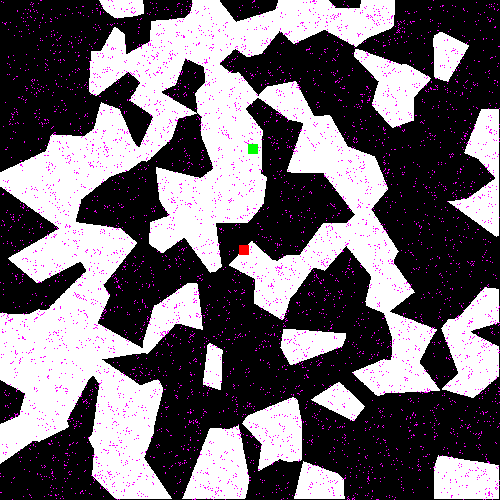
\includegraphics[scale=0.4]{../pictures/00000.png}
\end{figure}

\end{frame}

\begin{frame}{\bf Particle filter}

\begin{figure}[htbp]
  \centering
   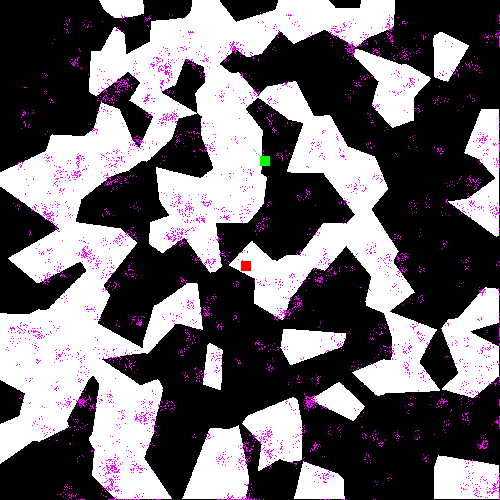
\includegraphics[scale=0.4]{../pictures/00010.png}
\end{figure}

\end{frame}

\begin{frame}{\bf Particle filter}

\begin{figure}[htbp]
  \centering
   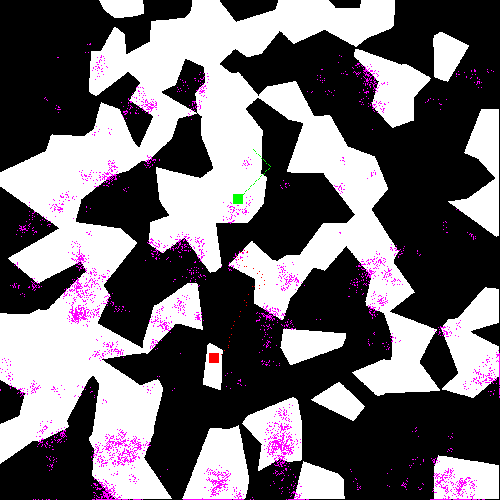
\includegraphics[scale=0.4]{../pictures/00040.png}
\end{figure}

\end{frame}

\begin{frame}{\bf Particle filter}

\begin{figure}[htbp]
  \centering
   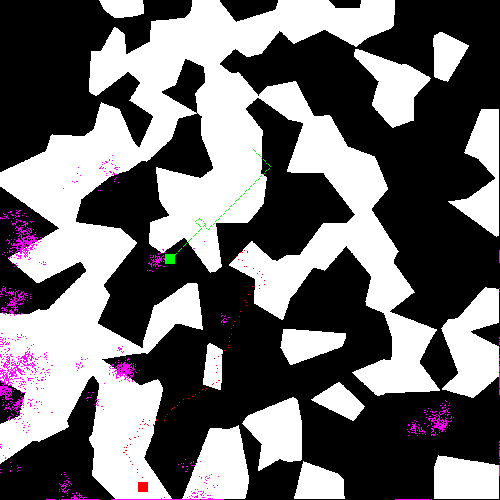
\includegraphics[scale=0.4]{../pictures/00110.png}
\end{figure}

\end{frame}

\begin{frame}{\bf Particle filter}

\begin{figure}[htbp]
  \centering
   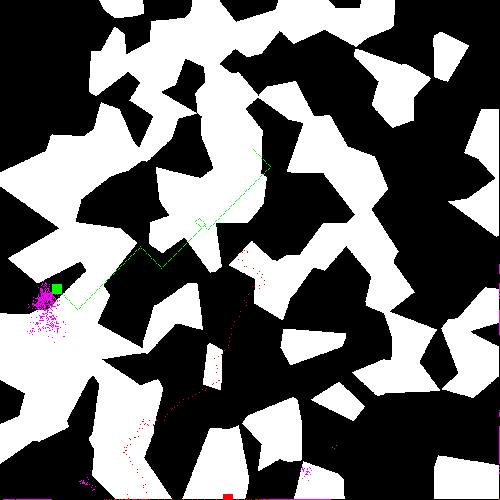
\includegraphics[scale=0.4]{../pictures/00200.png}
\end{figure}

\end{frame}

\begin{frame}{\bf Particle filter}

\begin{figure}[htbp]
  \centering
   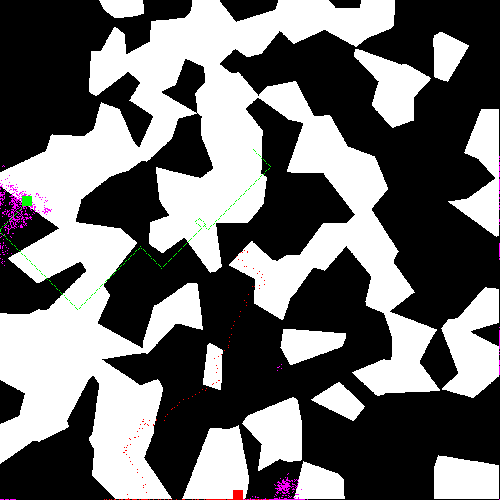
\includegraphics[scale=0.4]{../pictures/00270.png}
\end{figure}

\end{frame}


\begin{frame}{\bf Particle filter}

\begin{figure}[htbp]
  \centering
   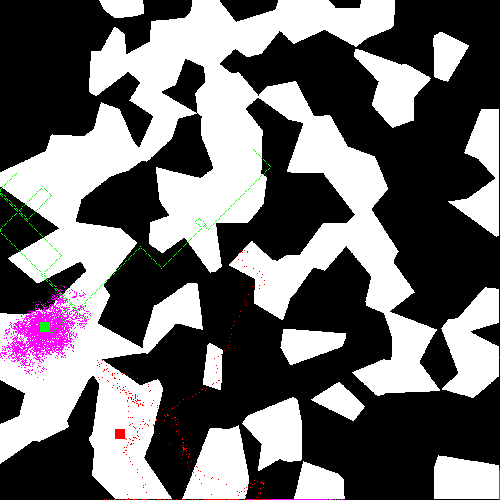
\includegraphics[scale=0.4]{../pictures/00500.png}
\end{figure}

\end{frame}


\begin{frame}{\bf Particle filter}

\begin{figure}[htbp]
  \centering
   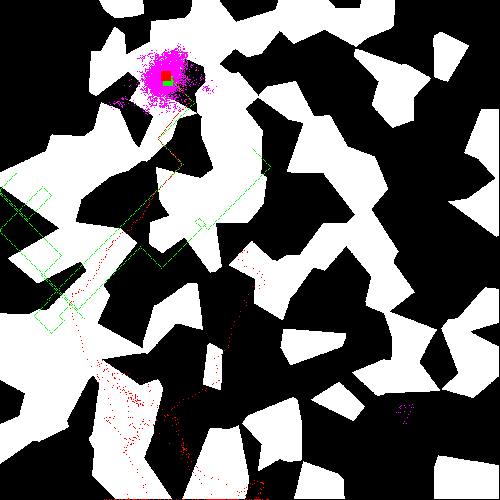
\includegraphics[scale=0.4]{../pictures/00700.png}
\end{figure}

\end{frame}


%-------------------------------------------------------------------------------------
\begin{frame}{\bf Q\&A}

\begin{figure}[ht]
\begin{center}
\begin{minipage}{0.8\linewidth}
\begin{center}
 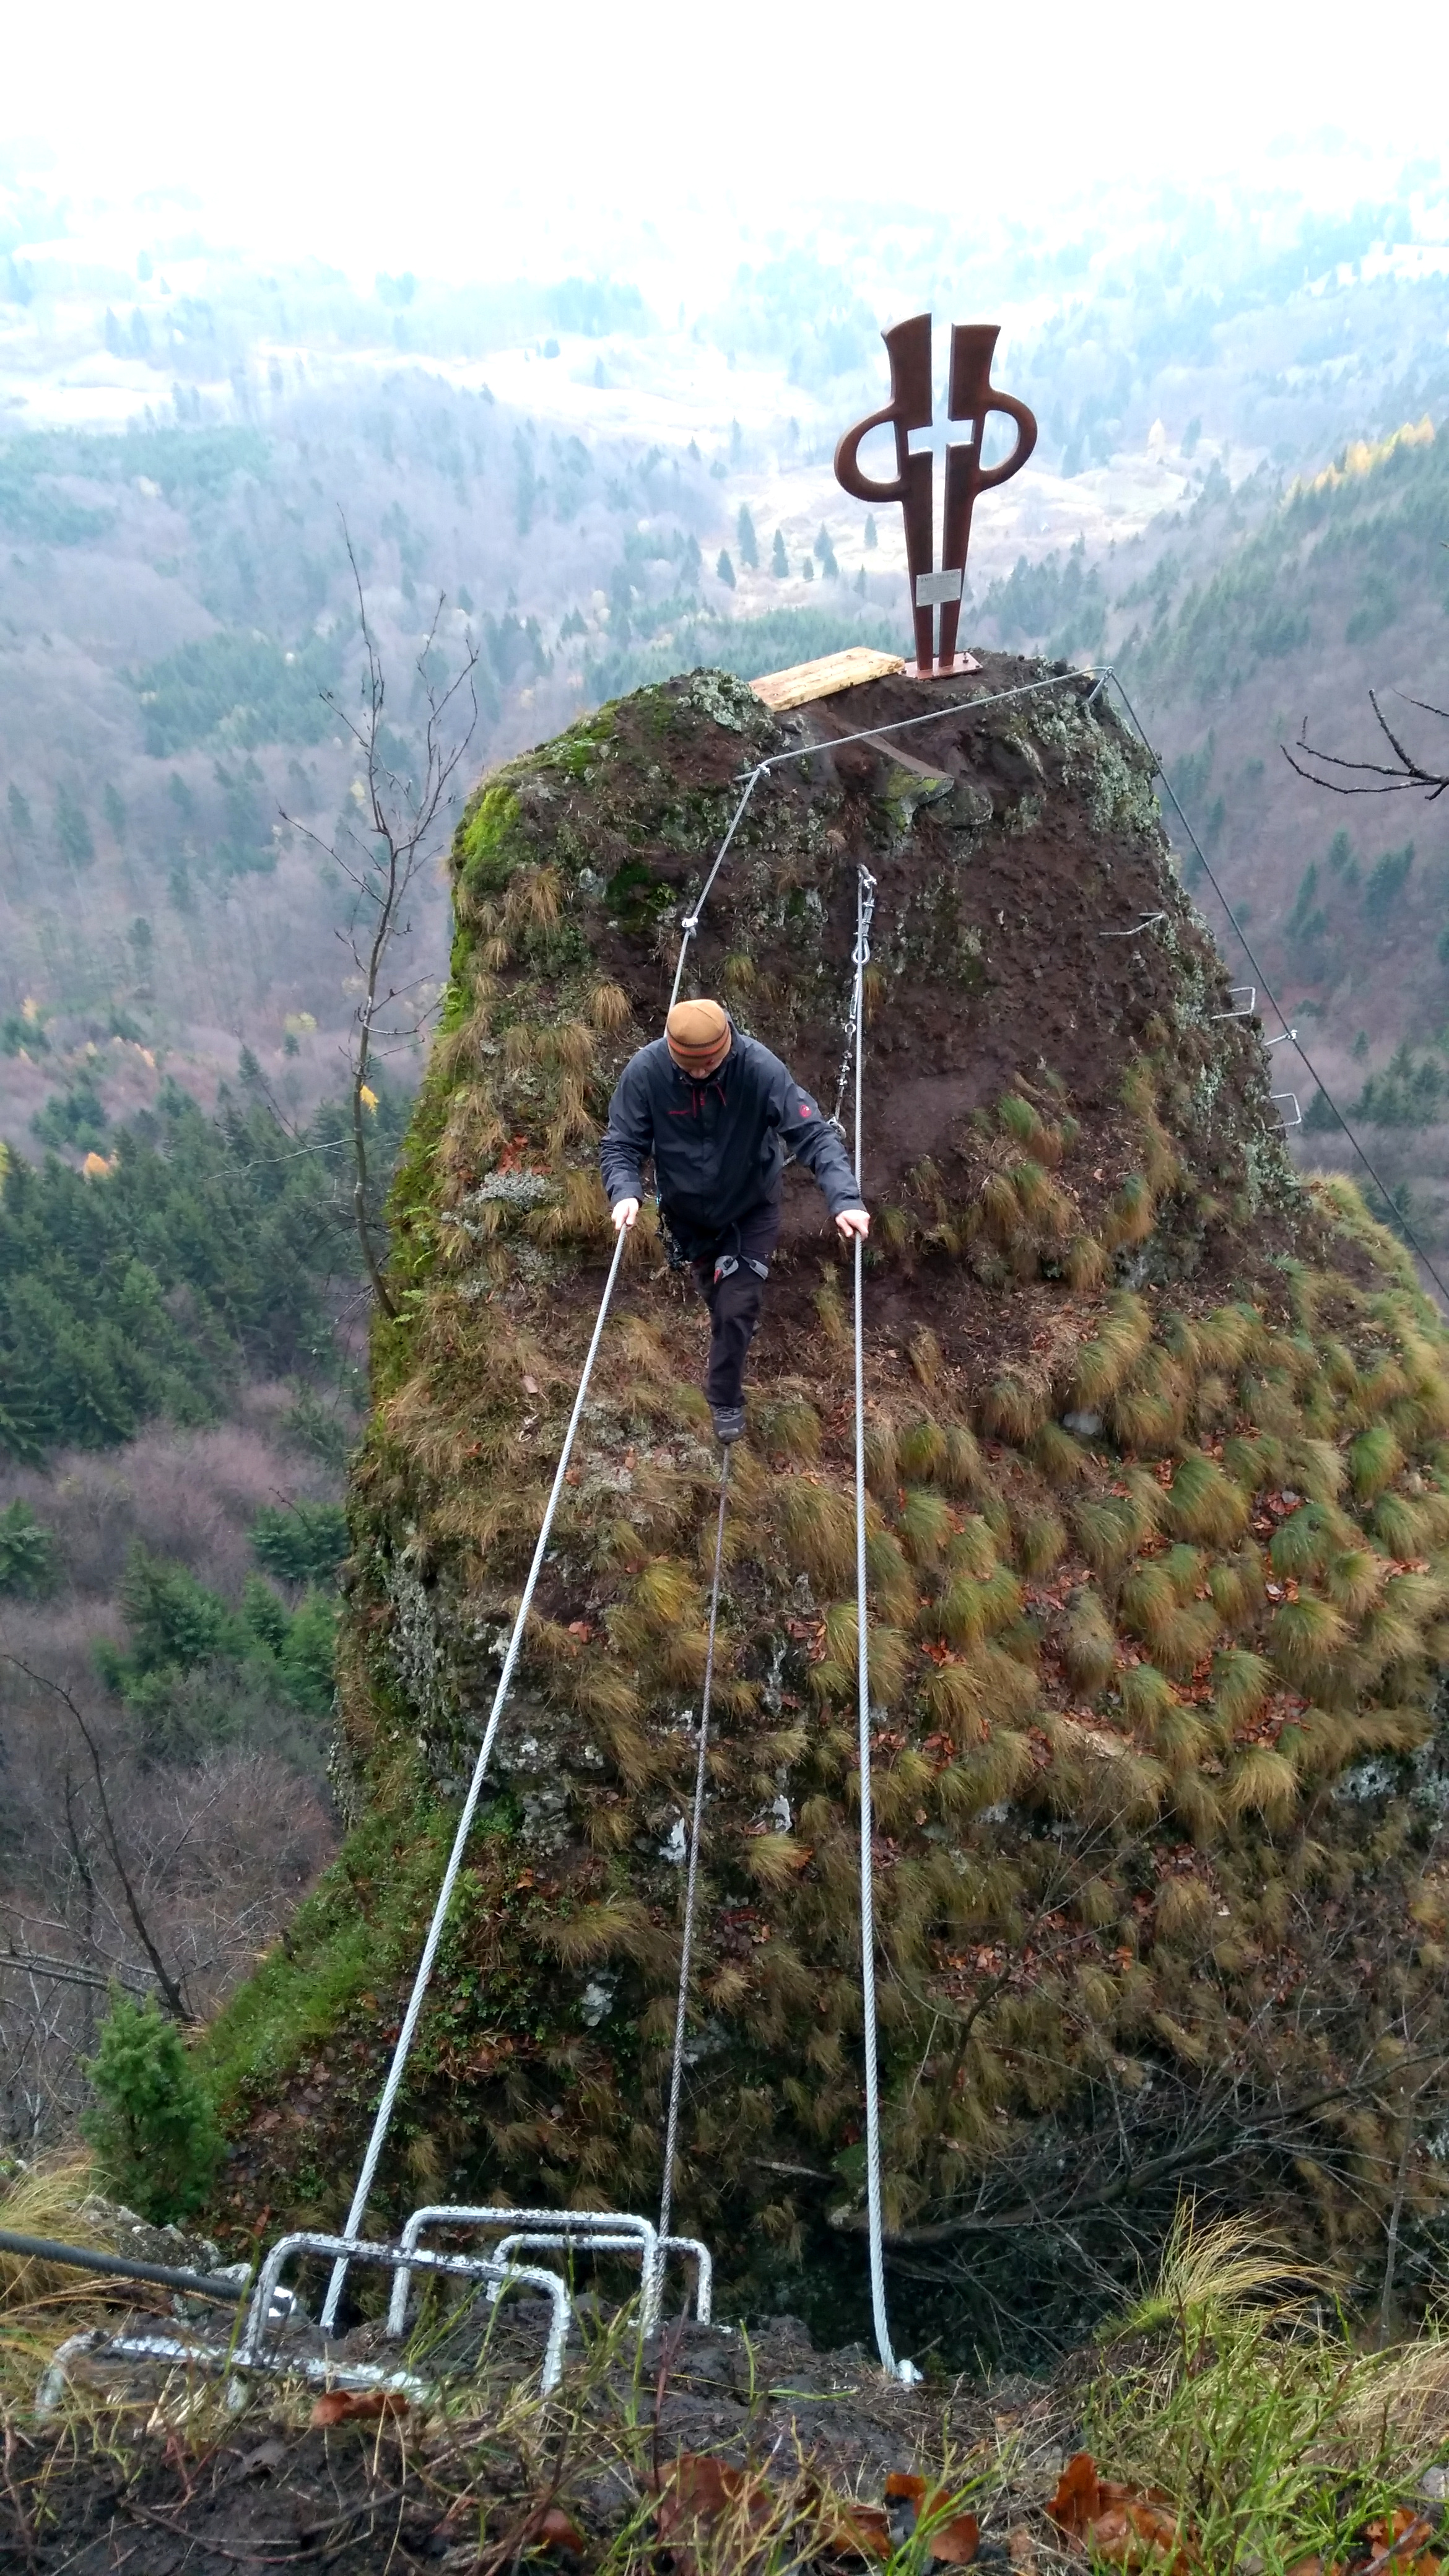
\includegraphics[width=0.4\textwidth]{../pictures/me2.jpg}
\end{center}
\end{minipage}
\end{center}
\end{figure}

\url{https://github.com/michalnand/robotics}
\url{https://github.com/michalnand/machine\_learning\_new}

\centerline{michal.nand@gmail.com}

\end{frame}

\end{document}
